\documentclass{article}
\usepackage[margin=1in]{geometry}

\usepackage{tikz,amsthm}
\usetikzlibrary{arrows,automata}
\newtheorem{theorem}{Theorem}
\newtheorem{lemma}{Lemma}
\title{CSCI 510, Fall 2016, Homework \# 1}
\author{SOLUTION SKETCHES}
\date{Due date: Tuesday, October 4, Midnight} 
%\newcommand{\duple}[2]{\left[\begin{array}{c} #1\\#2\end{array}\right]}
\newcommand{\duple}[2]{\left[{#1}\atop{#2}\right]}
\begin{document}
\maketitle
\begin{enumerate}
\item Transforming a NFA with $n$ states into a DFA may require as
  many as $2^n$ states.  Give examples of NFAs with 2 and 3 states
  that {\em require} 4 and 8 states, respectively, in their
  equivalent DFAs. Use the alphabet $\Sigma=\{0,1\}$.  Explain why
  they require $2^n$ states and find the DFAs in question.

  \begin{description}
  \item[2 states:] The NFA in Figure \ref{nfatwo} requires $2^n$
    states because there exist strings that lead to each possible
    subset in the power set of states:
    \\
    \begin{tabular}{cc}
      String & Leads to\\\hline
      $\varepsilon$ & $a$\\
      0 & $\emptyset$ \\
      1 & $b$\\
      10 & $a,b$
    \end{tabular}\\
    Further, none of these states can be eliminated from the resulting
    DFA since, in each state, there exist extensions of the current
    string that disagree on whether the current string is accepted or
    rejected. Therefore, none of the states are equivalent.  (For
    example, if $b$ had been the accepting state instead of $a$, then
    the states $b$ and $a,b$ in the resulting DFA would be equivalent,
    and could be merged.)

  \begin{figure}[!htbp]
    \begin{center}
  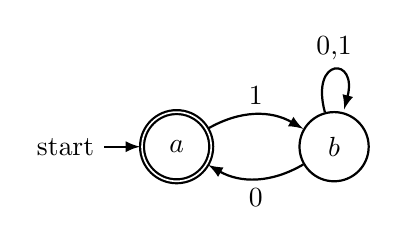
\begin{tikzpicture}[->,>=latex,thick,auto,node distance=2cm]
    \node[state,initial,accepting] (start){$a$};
    \node[state] (accept) [right of=start]{$b$};
    \path
    (start) edge [bend left] node {1} (accept)
    (accept) edge [loop above] node {0,1} (accept)
    (accept) edge [bend left] node {0} (start);
  \end{tikzpicture}
    \end{center}
    \caption{2-state NFA that requires 4 states for corresponding DFA.}
    \label{nfatwo}
  \end{figure}
  
  \begin{figure}[!htbp]
    \begin{center}
  \begin{tikzpicture}[->,>=latex,thick,auto,node distance=2cm]
    \node[state,initial,accepting] (a){$a$};
    \node[state] (b) [right of=start]{$b$};
    \node[state] (empty) [below of=a]{$\emptyset$};
    \node[state,accepting] (ab) [right of=empty]{$a,b$};
    \path
    (a) edge [] node {0} (empty)
    (a) edge [] node {1} (b)
    (b) edge [bend left] node {0} (ab)
    (b) edge [loop above] node {1} (b)
    (empty) edge [loop below] node {0,1} (empty)
    (ab) edge [loop below] node {1} (ab)
    (ab) edge [bend left] node {0} (b);
  \end{tikzpicture}
    \end{center}
    \caption{4-state DFA corresponding to 2-state NFA.}
    \label{dfatwo}
  \end{figure}

  \newpage

\item[3 states:]
The NFA is in Figure \ref{nfathree} and the DFA in Figure
\ref{dfathree}.  The argument for this machine is identical to the
argument for the previous case: there exists a unique string that
leads to each of the states in the DFA, and none of the states is
equivalent to any of the others because of the distribution of final
states. 

  \begin{figure}[!htbp]
    \begin{center}
  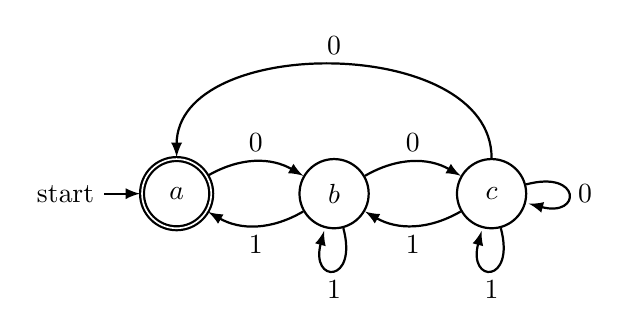
\begin{tikzpicture}[->,>=latex,thick,auto,node distance=2cm]
    \node[state,initial,accepting] (a){$a$};
    \node[state] (b) [right of=a]{$b$};
    \node[state] (c) [right of=b]{$c$};
    \path
    (a) edge [bend left] node {0} (b)
    (b) edge [bend left] node {0} (c)
    (b) edge [bend left] node {1} (a)
    (b) edge [loop below] node [below] {1} (b)
    (c) edge [bend left] node  {1} (b)
    (c) edge [loop below] node  {1} (c)
    (c) edge [loop right] node {0} (c)
    (c) edge [out=90,in=90] node [above] {0} (a)
;
  \end{tikzpicture}
    \end{center}
    \caption{3-state NFA that requires 8 states for corresponding DFA.}
    \label{nfathree}
  \end{figure}
  
  \begin{figure}[!htbp]
    \begin{center}
  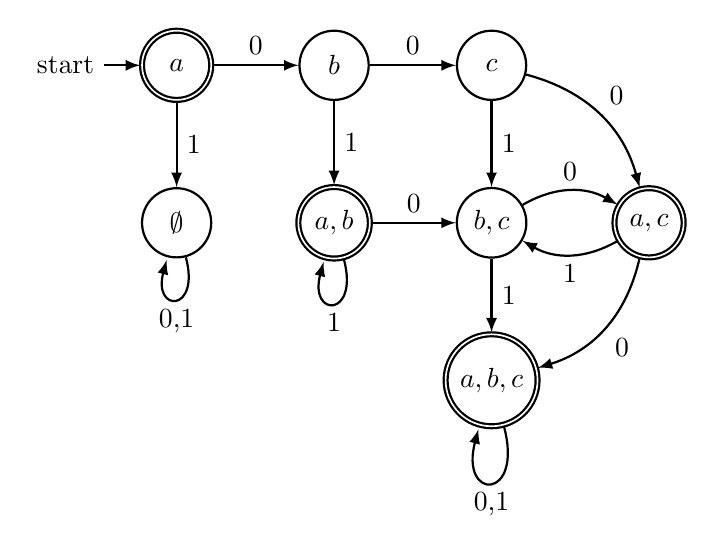
\begin{tikzpicture}[->,>=latex,thick,auto,node distance=2cm]
    \node[state,accepting,initial] (a){$a$};
    \node[state] (b) [right of=a]{$b$};
    \node[state] (c) [right of=b]{$c$};
    \node[state,accepting] (ab) [below of=b]{$a,b$};
    \node[state] (bc) [below of=c]{$b,c$};
    \node[state,accepting] (ac) [right of=bc]{$a,c$};
    \node[state] (empty) [below of=a]{$\emptyset$};
    \node[state,accepting] (abc) [below of=bc]{$a,b,c$};
    \path
    (empty) edge [loop below]  node {0,1} (empty)
    (a) edge node {0} (b)
    (a) edge node {1} (empty)
    (b) edge [] node {0} (c)
    (b) edge node {1} (ab)
    (c) edge node {1} (bc)
    (c) edge [bend left] node {0} (ac)
    (ab) edge node {0} (bc)
    (ab) edge [loop below] node {1} (ab)
    (bc) edge [bend left] node {0} (ac)
    (bc) edge node {1} (abc)
    (ac) edge [bend left] node {0} (abc)
    (ac) edge [bend left] node {1} (bc)
    (abc) edge [loop below] node {0,1} (abc)
;
  \end{tikzpicture}
    \end{center}
    \caption{8-state DFA corresponding to 3-state NFA.}
    \label{dfathree}
    \end{figure}
  \end{description}
    


\newpage
\item
  Let
  \[
  \Sigma=\left\{\duple{0}{0},\duple{0}{1},\duple{1}{0},\duple{1}{1}\right\}.
  \]
  So $\Sigma$ contains all columns of 0s and 1s of height two.  A
  string of symbols in $\Sigma$ give two rows of 0s and 1s.  Consider
  each row to be a binary number and let
  \[
  C = \{w\in\Sigma^* | \mbox{the bottom row is three times the top
    row}\}.
  \]
  For example, $\duple 00\duple 01 \duple 11 \duple 00\in C$ because
  the binary number 0110 is three times the binary number 0010,
  but
  $\duple 01 \duple01\duple10\not\in C$ because the binary number 110
  is not three times the binary number 001.  Show that $C$ is
  regular.

  For this problem you may assume the truth of the theorem that says
  that the reverse of a regular language is regular.  The reverse of a
  language $A$, written $A^R$, is the set of all strings
  $w^R=w_n\ldots w_2w_1$ such that $w=w_1w_2\ldots w_n\in A$,
  \[
  A^R = \{w^R |  \mbox{ $w^R=w_n\ldots w_2w_1$ where  $w=w_1w_2\ldots
    w_n\in A$}\},
  \]

  {\bf Solution.}
  Let's look at the process of multiplying a number by 3 in binary.
  In Figure \ref{multfig}, the carries are written as superscripts on the
  second line, for reasons that will be clear later.

  \begin{figure}[!htbp]
    \begin{center}
  \begin{tabular}{llllllll}
    &    1 & 0 & 0 & 1 & 1 & 1 & $\Leftarrow n$\\
    &    $\times$ &&&&1&1 & $\Leftarrow 3$\\\hline
    &    $1$ & $0$ & $0$ & $1$ & $1$ & $1$\\
     $1^0$ & $0^0$ & $0^1$ & $1^1$ & $1^1$ & $1^0$&\\\hline
     1& 1& 0& 0 &1 &0 &1 & $\Leftarrow 3n$\\
  \end{tabular}
  \end{center}
  \caption{Example of multiplying by 3 in binary.}
  \label{multfig}
  \end{figure}

  Basically we just shift the number one place to the left, and then
  add.  The first digit must be the same and cannot result in a carry.
  From there on, moving from right to left (taking advantage of the
  theorem that says we can do this right-to-left instead of
  left-to-right), at each position we can compute the answer by
  remembering what the bit to the right was (that will be the bit
  shifted to the left in the second row) and whether there was a carry
  from the previous addition.  For example, in the second column from
  the right, we need to remember that the shifted bit is a 1 and the
  carry bit is a 0.  In the second line this is written $1^0$.  In the
  third column, the shifted bit was a 1 and the carry was a 1.  We
  wrote this as $1^1$.

  To build our DFA, then, we will only need to remember two bits, and
  we need $2^2=4$ states for this.  One extra state will serve for the
  start state, and one other state as a permanent reject state if the
  two strings cannot be matched. (If we want to accept the empty
  string, we can dispense with the extra start state.)

  In Figure \ref{dfafig} we represent states as a circle with two bits
  in side, representing the pair (shifted bit, carry bit).  For
  example, the node \tikz{\node[state](foo){$0^1$}} represents a
  shifted bit of 0 and a carry bit of 1.  We can now add in the
  necessary transitions by following the laws of arithmetic.
Examples:
  \begin{itemize}
  \item     If we are in state $0^0$, and $n$ has a 0 in the next
  position, then $3n$ will also have a 0, and we will return to the
  state $0^0$, so the arc for $\duple 00$ goes from $0^0$ to $0^0$.
\item If we are in state $0^0$ and $n$ has a 1 in the next position,
  then $3n$ will have a 1 in this position, and we will end up
  with no carry, and a 1 as the shifted bit.   So the $\duple 11$ arc
  goes from $0^0$ to $1^0$.
  \end{itemize}

  Similarly,  we can fill out the entire
  transition function for our machine with this transition table:
  \\
  \begin{tabular}{cccc}
    State & $n$ bit & $3n$ bit & New state\\\hline
    $0^0$ & 0 & 0 & $0^0$\\
    $0^0$ & 0 & 1 & $\otimes$\\
    $0^0$ & 1 & 0 & $\otimes$\\
    $0^0$ & 1 & 1 & $0^0$\\\hline
    $1^0$ & 0 & 0 & $\otimes$\\
    $1^0$ & 0 & 1 & $0^0$\\
    $1^0$ & 1 & 0 & $0^0$\\
    $1^0$ & 1 & 1 & $\otimes$\\\hline
    $0^1$ & 0 & 0 & $\otimes$\\
    $0^1$ & 0 & 1 & $0^0$\\
    $0^1$ & 1 & 0 & $0^0$\\
    $0^1$ & 1 & 1 & $\otimes$\\\hline
    $1^1$ & 0 & 0 & $0^0$\\
    $1^1$ & 0 & 1 & $\otimes$\\
    $1^1$ & 1 & 0 & $\otimes$\\
    $1^1$ & 1 & 1 & $0^0$\\\hline
  \end{tabular}\\
  The accepting state has to have a carry of zero, and further the
  last bit of the $n$ string  must be a zero. If it were a 1, then
  there would be at least one more bit in the $3n$ string.  Thus,
  there is only one accepting state, namely $0^0$.
  The DFA that results from all of these considerations
  is shown in Figure \ref{dfafig}.

  It should be obvious from construction that this machine recognizes
  the language $C$, but we will sketch a more formal proof as follows:

  \begin{theorem} The language $C$ is identical to the language
    accepted by the DFA in Figure \ref{dfafig}.
  \end{theorem}
  \begin{proof}
This theorem will follow immediately from Lemmas \ref{lemma2} and
\ref{lemma3}, below.
    \end{proof}

  \begin{lemma}\label{lemma1}
    If a string $w$ with $|w|\geq 1$ is processed by the DFA, then at
    each point in the process if the state is not the trap state, then
    the state correctly represents both the previous bit of the $n$
    string, and the carry bit of a multiplicaiton of the $n$ string by
    3.  Further, if the state is the trap state, then $w$ cannot be in
    $C$.
    \end{lemma}
  \begin{proof}
This follows from the construction of the machine and induction.
    \begin{description}
      \item[Base:] The shortest possible strings are $\duple
        00, \duple 01, \duple10$, and $\duple11$.
        \begin{itemize}
          \item $\duple 01$ and $\duple10$ end up in the trap state,
            and neither one can be in $C$
          \item  $\duple00$ ends up in state $0^0$, and $\duple 11$
            ends up in state $1^0$, and both of these are correct.
        \end{itemize}
      \item[Step:] Suppose $|w|=n$ and all strings of length less than
        $n$ $w=w_nw_{n-1}\ldots w_1$.  Then by the inductive
        hypothesis the Lemma is true for the string $w_{n-1}\ldots
        w_1$.  By inspection of each case for $w_n$ in the transition
        function, above, the Lemma will also hold true for $w$.
    \end{description}
    
  \end{proof}

  \begin{lemma}\label{lemma2}
    If $w\in C$ then $w$ is accepted by the DFA.
  \end{lemma}
  \begin{proof}
    If $w\in C$ then by Lemma \ref{lemma1} it will not end up in the
    trap state.  Further, if $w\in C$ then the carry bit will be 0,
    and the last bit of the $n$ bitstream will be 0, then by Lemma
    \ref{lemma1} it will end up in state $0^0$, which is an accept state.
  \end{proof}

  \begin{lemma}\label{lemma3}
    If $w$ is accepted by the DFA, then $w\in C$.
  \end{lemma}
  \begin{proof}
If $w$ is accepted by the DFA, then  it will
finish in state $0^0$. By Lemma \ref{lemma1}, that implies that the
carry bit in a multiplication by 3 is 0, and also that the last bit of
the $n$ string is also 0.  This implies that the $3n$ string is the
bit representation of the number $3n$.
  \end{proof}

  \begin{figure}[!htbp]
    \begin{center}
  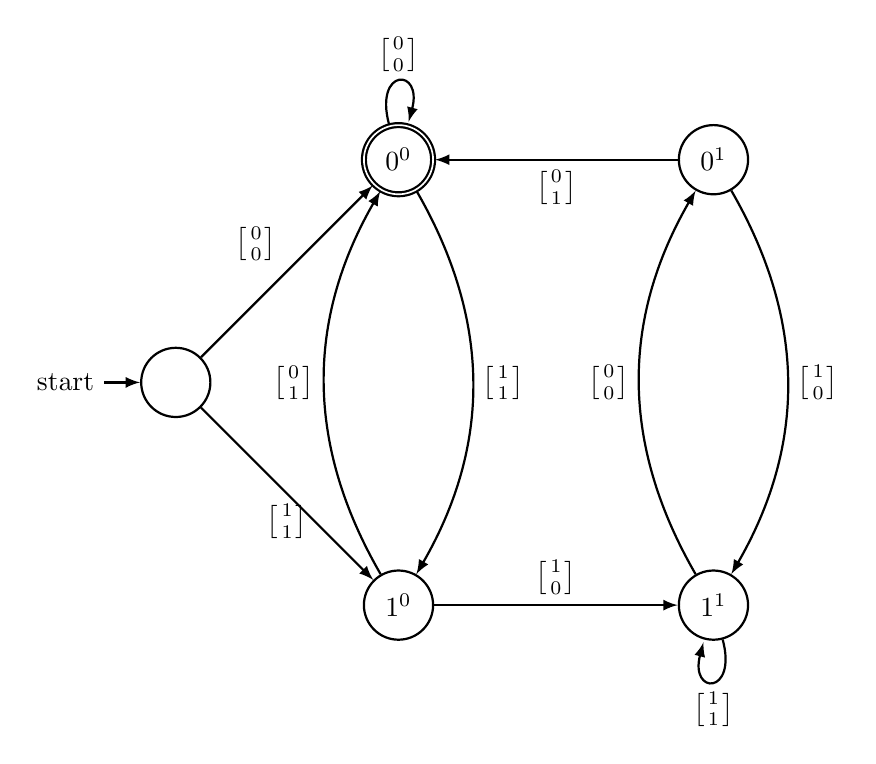
\begin{tikzpicture}[->,>=latex,thick,auto,node distance=4cm]
    \node[state,initial] (start){};
    \node[state,accepting] (00) [above right of=start]{$0^0$};
    \node[state] (01) [right of=00] {$0^1$};
    \node[state] (10) [below right of=start] {$1^0$};
    \node[state] (11) [right of=10] {$1^1$};
    \path
    (start) edge node {$\duple 00$} (00)
    (start) edge node [below] {$\duple 11$} (10)
    (00) edge [loop above] node {$\duple 00$} (00)
    (00) edge [bend left] node {$\duple 11$} (10)
    (10) edge [bend left] node {$\duple 01$} (00)
    (10) edge [] node {$\duple 10$} (11)
    (11) edge [bend left] node {$\duple 00$} (01)
    (11) edge [loop below] node {$\duple 11$} (11)
    (01) edge [] node {$\duple 01$} (00)
    (01) edge [bend left] node {$\duple 10$} (11);
  \end{tikzpicture}
    \end{center}
    \caption{DFA for the $n/3n$ problem.  Transitions that go to the
      trap state are omitted for clarity.  Note:  states $0^1$ and $1^0$ can
    be collapsed into one state.  We only really need to remember whether 0, 1, or 2 needs to be carried into the sum.}
    \label{dfafig}
    \end{figure}



\newpage
\item Let $\Sigma$ be as in the previous problem, and let
  \[
  E=\{w\in\Sigma^*|\mbox{the bottom row of $w$ is the reverse of the
    top row of $w$}\}.
    \]
    Show that $E$ is not regular.
\end{enumerate}
\end{document}
